\documentclass[ENG]{TFUOC}%IB: CASTELLÀ, CAT: CATALÀ, ENG: ANGLISH

%Introduce Work Data
\title{Title of the complete and as long work as necessary}
\titcrt{Very short title} %Short title to appear in header
\author{Salomon Elieser Marquez Villalobos}
\date{September 21, 2021}


\nomPDC{Tutor Tutor Name}
\nomPRA{Appoint Responsible Teaching Staff}
\titulac{Master in XXX}
\area{Work Area}
\idioma{Catalan}
\credits{15}
\parcla{word, key, work}

\licenc{ccBy}
%Possible licenses
%ccByNcNd
%ccByNcSa
%ccByNc
%ccByNd
%ccBySa
%ccBy
%GNU
%copyright


%%%%%%%%%%
% Summary in language

\abstractidioma{
Maximum 250 words, for the purpose, context of application, methodology, results and conclusions of the work.
}

% Summary in English.
\abstractenglish{
A maximum of 250 words, detailing the purpose, context of application, methodology, results and conclusions of the work.
}

\begin{document}

\estructura

\tableofcontents

\listoffigures

\listoftables




\chapter{Introduction}

This template is conceived as a guide for the student. It can be adapted to the needs of each work, provided that the tutor of the work agrees.

\section{Context and justification of work}


Work starting point (What is the need to cover? Why is it a relevant issue? How is the problem solved at the moment?) and contribution made (What result do you want to obtain?).

It is important to bear in mind that the final work must be understandable for anyone who knows the area of knowledge, but does not have to be an expert in the subject of what the work is about.

\section{Work objectives}

List of objectives of the work.

\section{Impact on sustainability, ethics-social and diversity}
\label{s:etic}

This section should identify the positive and/or negative impacts of the final project on the three dimensions of UOC's cross-disciplinary competence "Ethical and global commitment".
 
The Cross-cutting Guide on Ethical and Global Competence will help you write these sections.


\section{Focus and method followed}

Mention of what are the possible strategies to carry out the work and what is the chosen strategy (develop a new product, adapt an existing product...). It is necessary to include an assessment of why this is the most appropriate strategy to achieve the objectives.   	



\section{Work schedule}

Description of the necessary resources to do the work, the tasks to be carried out and a temporary planning of each task using a Gantt diagram or similar. This planning should mark the partial milestones of each of the CAPs.



\section{Brief summary of products obtained}

No need to go into detail: the detailed description will be made in the rest of the chapters.

%It is not necessary to enter in detail: the detailed description will be done in the rest of the chapters.

\section{Brief description of other memory chapters}

Brief explanation of the contents of each chapter and its relationship with the global project.

%\chapter{State of Art}

%State of the art of the subject in question. It should end up showing why work is important and contributes something, and with the hypotheses of work.

\chapter{Materials and methods}
In these sections, it is necessary to describe:
\begin{itemize}
    \item The most relevant aspects of the design and development of the work.
    \item The methodology chosen to carry out this development, describing the possible alternatives, the decisions taken, and the criteria used to make these decisions.
    \item The products obtained.
\end{itemize}

 
\textbf{Chapter structuring may vary depending on the type of work.}  
 
If applicable, a section on “Economic evaluation of work” will be included. This section will indicate the expenses associated with the development and maintenance of work, as well as the economic benefits obtained and a final analysis on the viability of the product.



\chapter{Results}

Detail in this section the results obtained using the methodology described in the previous section.


%Recull of job results. There should be a correspondence with the methodology that the results are what is obtained after applying the methodology.

The figures must be explained and quoted in the text, such as \ref{fig:my_label}, in which the error is shown depending on the distance, in arbitrary units. All graphs must have the title of the axes.

\begin{figure}[!htbp]
    \centering
    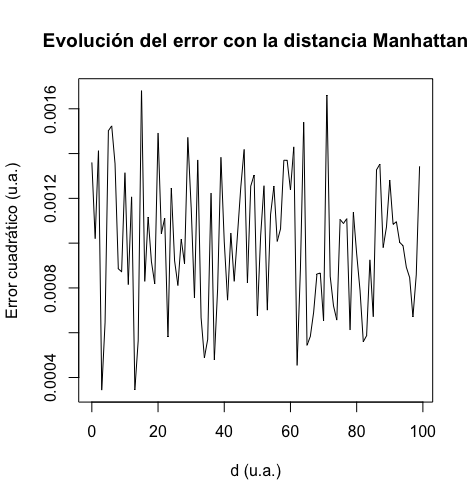
\includegraphics[width=7truecm]{Rplotmanh.png}
    \caption{Error working distance in arbitrary units.}
    \label{fig:my_label}
\end{figure}

%\chapter{Discussion}
%Discussion of results in project context. It is in this section that they make sense and in which the research questions are answered and it is shown how the results respond to the problems raised.

%This part may not apply depending on the type of work.

%\chapter{Economic evaluation}
%If applicable, a section of ``Economic evaluation of work' will be included. This section will indicate the expenses associated with the development and maintenance of work, as well as the economic benefits obtained. A final analysis on the viability of the product must be carried out.

\chapter{Conclusions and future works}

%\section{Conclusions}
This chapter must include:
\begin{itemize}
\item A description of the conclusions of the work:
\begin{itemize}
    \item Once the results have been obtained, what conclusions are drawn?
    \item Are these results as expected? Or have they been amazing? Why?
\end{itemize}
\item A critical reflection on the achievement of the objectives initially set:
\begin{itemize}
    \item Have we achieved all the objectives? If the answer is negative, why?
\end{itemize}
\item A critical analysis of the monitoring of planning and methodology throughout the product:
\begin{itemize}
    \item Has the schedule been followed?
    \item Has the planned methodology been adequate enough?
    \item Has it been necessary to introduce changes to ensure the success of the work? Why?
\end{itemize}
\item From the impacts foreseen in \ref{s:etic}, ethical-social, sustainability and diversity, evaluate/mention whether they have been mitigated (if they were negative) or whether they have been achieved (if they were positive). 
\item If unforeseen impacts have appeared in \ref{s:etic}, evaluate/mention how they have mitigated (if they were negative) or what they have contributed (if they were positive).
\item The future lines of work that have not been explored in this work and have remained pending.


%\item A description of the conclusions of the work: What lessons have been learned from work?
%\item A critical reflection on the achievement of the objectives initially set: Have we achieved all the objectives? If the answer is negative, why?
%\item Of the impacts foreseen in the section \ref{s:etic}, an assessment, or at least mention, of whether they have been mitigated (if they were negative) or whether they have been achieved (if they were positive). 
\end{itemize}

%\section{Future Lines}
%The future lines of work that could not be explored in this work and have been pending.

%\section{Schedule Tracking}
%A critical analysis of the monitoring of the planning and methodology throughout the work: 
%\begin{itemize}
%    \item  Have the schedule been followed? 
%    \item Has the planned methodology been adequate? 
%    \item Has it been necessary to introduce changes to ensure the success of the work? Why?
%\end{itemize}

\chapter{Glossary}

Definition of the most relevant terms and acronyms used in the Report.

%Defining the most relevant terms and acronyms used within the Memory.

\chapter{Bibliography}

Numbered list of bibliographic references used within memory. In each place where a reference is used within the text, it must be indicated by quoting the reference number, for example: [7].

It is very important to include all the references used and quote them appropriately, that is, including all the information necessary to identify the reference. The minimum information to be included according to the reference type is:

\begin{itemize}
\item Book: Authors, Title, Edition (if applicable) Editorial, City, Year.
\item  Journal article: Authors, Title, Name of the Journal, Home and End Page Number, Issue of the magazine / Volume, Year.
\item  Web: URL and date it was visited.
\end{itemize}

Information on how to quote documents: \url{http://biblioteca.uoc.edu/es/recursos/citacion-bibliografica}.


\newpage
\appendix
List of sections that are too extensive to include in memory and have a self-contained character (e.g. user manuals, installation manuals, etc.)
 
Depending on the type of work, there may be no need to add an annex.

\end{document}
